\section{流形上的优化问题}
\label{sec:mfo-problems}

什么样的约束集合可以当作计算空间？本节先看两个具体约束，指出它们共有的结构，再说明这一结构在哪些集合上不存在。

\paragraph{两个具体约束}
球面约束$\bm{x}^\top\bm{x}=1$只有一个方程。从点$\bm{x}$出发沿曲线$\bm{c}(t)$运动，并一直留在球面上，就要求$\bm{c}(t)^\top\bm{c}(t)=1$。对$t$求导并取$t=0$，得到速度$\bm{v}=\bm{c}'(0)$必须满足
\[
 \bm{x}^\top\bm{v}=0.
\]
因此$\bm{x}$处允许的运动方向是与$\bm{x}$垂直的全体向量，构成一个$n-1$维的线性子空间。

矩阵约束$\bm{X}^\top\bm{X}=\bm{I}_k$的方程更多。这里$\bm{X}\in\mathbb{R}^{n\times k}$，$k\leq n$，它的列是一组标准正交向量。同样沿曲线$\bm{C}(t)$求导，速度$\bm{\Delta}=\bm{C}'(0)$必须满足
\[
 \bm{X}^\top\bm{\Delta}+\bm{\Delta}^\top\bm{X}=\bm{0}.
\]
这个条件说的是$\bm{X}^\top\bm{\Delta}$是反对称矩阵。例如$n=3$，$k=2$时，矩阵有$6$个元素，约束有$3$个独立方程，所以允许的方向构成一个$3$维子空间。

两个例子的共同点是：约束对变量的允许变化作出限制，而这个限制在每一点都是一个线性子空间，维数处处相同。这正是后面所有方法的立足点，在每一点都有一张平坦的“工作台”，可以在上面做线性代数。

\paragraph{正则等式约束给出流形}
把上面的观察写成一般形式。设$h:\mathbb{R}^n\to\mathbb{R}^p$光滑，可行集是它的零点集：
\begin{equation}
 M=\{\bm{x}\in\mathbb{R}^n:\ h(\bm{x})=\bm{0}\}.
 \label{eq:mfo-level-set}
\end{equation}
记$\bm{J}(\bm{x})$为$h$在$\bm{x}$处的Jacobian矩阵，假定它在$M$的每一点都行满秩。这就是第~\ref{chap:constrained-optimality}章的线性无关约束规范，这里要求它在整个可行集上成立。

这个条件保证$M$是$n-p$维的嵌入子流形，切空间就是Jacobian的零空间：
\begin{equation}
 T_{\bm{x}}M=\ker\bm{J}(\bm{x}).
 \label{eq:mfo-tangent}
\end{equation}
这里用到的是正则水平集定理及切空间的刻画，可参考\BookChapterRef{chap:manifold-relations}{卷四第26章“流形之间的关系”}。球面取$h(\bm{x})=\bm{x}^\top\bm{x}-1$，$\bm{J}(\bm{x})=2\bm{x}^\top$在球面上不为零；矩阵约束取值于对称矩阵，同样满足这个条件。

流形上的优化问题写作
\begin{equation}
 \min_{\bm{x}\in M}\ f(\bm{x}),
 \label{eq:mfo-problem}
\end{equation}
其中$f$定义在包含$M$的开集上并且光滑。本章把$M$就当作前面各章的可行集$\bm{C}$，并沿用卷四的写法把流形记成$M$，把球面记成$S^{n-1}$，把正交列矩阵的集合记成Stiefel流形$\mathrm{St}(k,n)$。问题本身仍是约束极值，改变的只是求解时使用的计算空间。

\paragraph{集合、度量与表示}
“在流形上计算”牵涉三个不同的选择，混淆它们会带来错误的结论。集合$M$由问题决定，它规定了哪些点可行，哪些点是极小点。

\term{黎曼度量}（Riemannian metric）是在每个切空间放一个内积，记为$\langle\bm{u},\bm{v}\rangle_{\bm{x}}$。同一个集合可以配不同的度量。度量决定长度和角度，因而决定“最陡”的方向，但不改变极小点的位置。本章除特别说明外，都取欧氏内积限制到切空间上的诱导度量。

表示方式是在计算机里怎样存一个点。球面上的点可以存成三个坐标，也可以存成两个角度；一个子空间可以存成任意一组基，这时同一个对象有许多矩阵记录。表示决定存储和运算的代价，第~\ref{sec:mfo-representation}节专门讨论。表~\ref{tab:mfo-three-choices}把三者并列。

\begin{BookInlineTable}
 \centering
 \caption{流形优化中三种不同的选择。}
 \label{tab:mfo-three-choices}
 \begin{tabular}{lll}
  \toprule
  选择 & 决定什么 & 不决定什么\\
  \midrule
  集合$M$ & 可行点、极小点 & 梯度的数值\\
  度量$\langle\cdot,\cdot\rangle_{\bm{x}}$ & 梯度、Hessian、步长的尺度 & 极小点的位置\\
  表示 & 存储和运算成本 & 所求的几何对象\\
  \bottomrule
 \end{tabular}
\end{BookInlineTable}

\paragraph{带奇点或棱角的集合}
前面的立足点并非总存在。图~\ref{fig:mfo-regular-singular}对比了三种集合。圆周上每点都有一条切线，法向量$\nabla h$不为零，这是正则的情形。

\begin{BookInlineFigure}
 \centering
 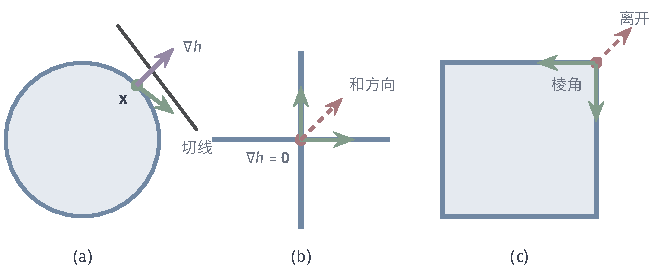
\includegraphics[width=111.9mm]{figures/05-optimization/06-constrained-optimization/tikz/mfo-regular-singular/figure.pdf}
 \caption{三种约束集合。(a)~圆周处处正则，切方向（绿）构成一条直线，紫箭头是约束的梯度。(b)~十字形$x_1x_2=0$在原点处约束梯度为零，两个绿色可行方向之和（红虚线）不可行，可行方向不构成线性子空间。(c)~正方形的角点处，可行方向只有一个锥，朝外的方向（红虚线）不可行。}
 \label{fig:mfo-regular-singular}
\end{BookInlineFigure}

十字形$\{x_1x_2=0\}$在原点处有两条可行的直线，把两个可行方向相加却得到不可行的方向，所以那里没有一个线性的切空间。这里$\nabla(x_1x_2)$在原点为零，正则条件不成立。

棱角的情形类似。方形可行域的角点处，允许的方向只构成一个锥，负向不再允许。这类可行集要用第~\ref{chap:feasible-iterations}章的投影或第~\ref{chap:penalty-multiplier-methods}章的乘子方法，本章的迭代不能直接套用，因为后面每一步都假定当前点处有一个完整的线性切空间。
